\documentclass[%
%draft,
11pt,%
twoside,%
titlepage,%
german,%
headsepline%
]{scrartcl}

\usepackage{lastpage}
\usepackage{amsthm}
\usepackage{amssymb}
\usepackage{geometry}
\usepackage{graphicx}
\usepackage[dvipsnames]{xcolor}
\usepackage[utf8]{inputenc}
\usepackage[ngerman]{babel}
\usepackage{lscape}
\usepackage[framemethod=TikZ]{mdframed}
\usepackage[most]{tcolorbox}
\usepackage{enumerate}
\usepackage{units}
\usepackage{nicefrac}
\usepackage{pgf,tikz}
\usetikzlibrary{arrows}
\usetikzlibrary{arrows.meta}
\usetikzlibrary{patterns}
\usetikzlibrary{positioning}
\usetikzlibrary{shadows}
\usepackage{colortbl}
\usepackage{hhline}
\usepackage{multirow}
\usepackage[extendedchars]{grffile}
\usepackage{caption}
\usepackage{multicol,calc}
\usepackage{blindtext}
\usepackage{pdfpages}
\usepackage{hyperref}
\usepackage{framed}

\usepackage{marginnote}
\usepackage{qrcode}
\qrset{height=9ex}

\usepackage{longtable}
\usepackage{listings}
\usepackage{wrapfig}

\usepackage{fontawesome} % Oder FontAwesome, falls du ein Augensymbol aus einer
\newcommand{\faEyeLightGray}{\textcolor{lightgray}{\faEye}} % Custom command for the gray eye icon

% package für plots mit dem Befehl axes
\usepackage{pgfplots}



% Command, um Tabellen-Spalten anzupassen
\newcommand{\spaltenheight}{\rule{0mm}{3ex}}
\newcommand{\spaltenwidth}{\rule{3cm}{0mm}}
\newcommand{\spaltensep}{\\[1ex]}
%\arrayrulecolor{darkgreen}
\doublerulesepcolor{white}

% colors
\definecolor{lightyellow}{rgb}{1,1,0.8}
\definecolor{Gray}{gray}{0.9}
\definecolor{lightgray}{rgb}{0.7, 0.7, 0.7}
\definecolor{darkblue}{rgb}{0,0,0.55}
\definecolor{firebrick}{rgb}{0.7,0.13,0.13}
\definecolor{seagreen}{rgb}{0.18,0.55,0.34}
\definecolor{emerald}{HTML}{50C878} % color of Definition
\definecolor{whitesmoke}{HTML}{F5F5F5} % background for environments
\definecolor{myblizzardblue}{HTML}{87CEEB} % color of Satz

% Für Definitionen im Fliesstext
\newcommand{\definition}[1]{\colorbox{emerald}{#1}}
% Geogebra-Link
\newcommand{\geogebralink}{\href{https://www.geogebra.org/calculator}{\texttt{geogebra.org}}}

% Umgebungen
\theoremstyle{definition}
    \newtheorem{bsp}{Beispiel}[subsection] % Beispiele
    \newtheorem{bem}{Bemerkung}[subsection] % Bemerkungen
\theoremstyle{plain}
    \newtheorem{thm}{Theorem} % Theorem [subsection]
    \newtheorem{satz}{Satz} % Satz [subsection]

% Umgebung lsg mit dynamischer Referenzierung und Label
\newcommand{\concatueb}[1]{ueb:#1}% Definition für concatueb
\newcommand{\concatlsg}[1]{lsg:#1}% Definition für concatlsg

\newcounter{uebcounter}[section]
\renewcommand{\theuebcounter}{\thesection.\arabic{uebcounter}}  % Zählerformat: Abschnitt.Übung

\newenvironment{lsg}[1]{%
    \par\noindent\textbf{Notizen zu Übung \ref{\concatueb{#1}}.}%
    \label{\concatlsg{#1}}
}{%
    \par%
}

\newenvironment{uebenv}[1]{%
    \refstepcounter{uebcounter}
    \par\noindent\textbf{Übung \theuebcounter.}%
    \label{\concatueb{#1}}\hfill\hyperref[\concatlsg{#1}]{\faEyeLightGray}\par
}{%
    \par
}

% Umgebung für Definitionen
\newcounter{deff}[section]\setcounter{deff}{0}
\renewcommand{\thedeff}{\arabic{section}.\arabic{deff}}

\newenvironment{cdef}[1][]{%
    \refstepcounter{deff} 
    \ifstrempty{#1}%
    % if condition (without title)
    {\mdfsetup{%
        frametitle={%
            \tikz[baseline=(current bounding box.east),outer sep=0pt]
            \node[anchor=east,rectangle,fill=emerald]
            {\strut Definition~\thedeff};}
        }%
    % else condition (with title)
    }{\mdfsetup{%
        frametitle={%
            \tikz[baseline=(current bounding box.east),outer sep=0pt]
            \node[anchor=east,rectangle,fill=emerald]
            {\strut Definition~\thedeff:~#1};}%
        }%
    }%
% for both conditions
    \mdfsetup{%
        innertopmargin=10pt,linecolor=emerald,%
        backgroundcolor=whitesmoke,%
        linewidth=2pt,topline=true,%
        frametitleaboveskip=\dimexpr-\ht\strutbox\relax%
    } 
\begin{mdframed}[]\relax}{%
\end{mdframed}}

% Farbig umrahmte Umgebung Satz
\newcounter{satzz}[section]\setcounter{satzz}{0}
\renewcommand{\thesatz}{\arabic{section}.\arabic{satzz}}

\newenvironment{csatz}[1][]{%
    \refstepcounter{satzz}
 
    \ifstrempty{#1}%
    % if condition (without title)
    {\mdfsetup{%
        frametitle={%
            \tikz[baseline=(current bounding box.east),outer sep=0pt]
            \node[anchor=east,rectangle,fill=myblizzardblue]
            {\strut Satz~\thesatz};}
        }%
    % else condition (with title)
    }{\mdfsetup{%
        frametitle={%
            \tikz[baseline=(current bounding box.east),outer sep=0pt]
            \node[anchor=east,rectangle,fill=myblizzardblue]
            {\strut Satz~\thesatz:~#1};}%
        }%
    }%
% for both conditions
    \mdfsetup{%
        innertopmargin=10pt,linecolor=myblizzardblue,%
        backgroundcolor=whitesmoke,%
        linewidth=2pt,topline=true,%
        frametitleaboveskip=\dimexpr-\ht\strutbox\relax%
    }
\begin{mdframed}[]\relax}{%
\end{mdframed}}

% kein Einzug bei neuem Abschnitt
\setlength{\parindent}{0pt} \setlength{\parskip}{1em}
\pagestyle{headings} % gemachte Einstellungen anwenden

\subject{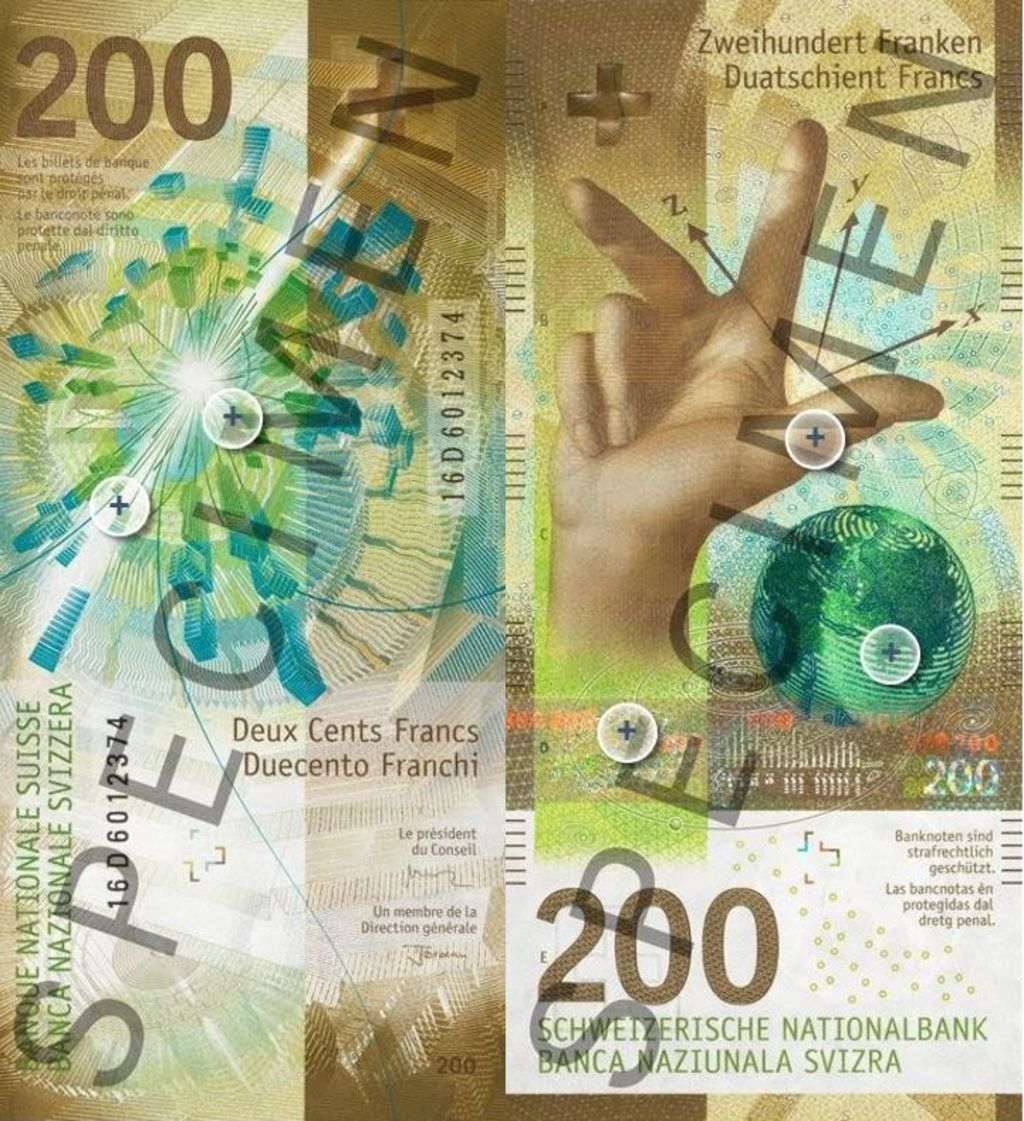
\includegraphics[width=0.618\textwidth]{pictures/200er}}
\title{Vektoren}
\subtitle{Raus in den 3D}
\author{}
\date{}
\lowertitleback{
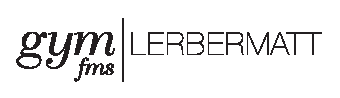
\includegraphics[height=1cm]{pictures/gymfmslerbermattlogo.eps}
\hfill%\copyright%
{\begin{tikzpicture}
  % Draw the rounded rectangle and clip the image to it
  \clip [rounded corners=5mm] (0,0) rectangle (1,1); % Adjust dimensions as needed
  \node at (0.5,0.5) {\includegraphics[width=1cm]{pictures/teacher_me_caricatur.png}}; % Adjust width and center image
\end{tikzpicture}}
}

\begin{document}
\maketitle
\tableofcontents
%\thispagestyle{empty}
\cleardoublepage
%\setcounter{page}{1}

\clearpage

\section{Produkte}
\subsection{Das Skalarprodukt}

Es ist zweckmässig eine Verknüpfung zweier vektorieller Grössen $\vec{v}$ und $\vec{w}$ einzuführen, so dass das Ergebnis ein Skalar ist. Offensichtlich wird das Ergebnis vom Winkel gebildet durch $\vec{v}$ und $\vec{w}$ abhängen. Wünschenswert wäre also eine Formel, mit der man den Winkel zwischen zwei Vektoren direkt berechnen kann.

\begin{ueb}[Herleitung Zwischenwinkel]\label{skalarprodukt}
Zeichne
\marginnote{
\qrcode{
https://www.youtube.com/watch?v=h5c7jdPZoWI}
}
ein beliebiges Dreieck und wähle zwei Seiten als $\vec{v}$ bzw. $\vec{w}$. Drücke die dritte Seite als Differenz dieser beiden Vektoren aus und formuliere mit allen dreien den Cosinussatz. Vereinfache danach und löse nach dem Winkel auf.
\end{ueb}

\begin{bem}
Diese Herleitung liefert also die gesuchte Formel, aus der der Zwischenwinkel zweier Vektoren berechnet werden kann. Ferner taucht bei der Herleitung der Term
$$v_xw_x+v_yw_y+v_zw_z$$
auf. Da dieser Ausdruck in der Vektorrechnung häufig auftritt und Anwendung in den Naturwissenschaften findet, hat man eine kürzere Schreibweise eingeführt und ihm einen Namen gegeben.
\end{bem}

\begin{cdef}[Skalarprodukt]{}
Das
\marginnote{
\qrcode{
https://m.youtube.com/watch?v=64AHlh8jFzo}
}
\textbf{Skalarprodukt} zweier Vektoren $\vec{v}$ und $\vec{w}$ ist definiert durch
$$\vec{v}\cdot\vec{w}=v_xw_x+v_yw_y+v_zw_z.$$
\end{cdef}
\begin{bem}
Mit Freude stellen wir fest, dass die verrichtete Arbeit mit dem Skalarprodukt ohne Trigonometrie und Berechnung des Zwischenwinkels bestimmt werden kann. Es gilt nämlich
$$W=\V{F}\cdot\V{s}$$
\end{bem}
Mit Hilfe des Skalarprodukts lässt sich der Winkel $\varphi$ zwischen zwei Vektoren $\vec{v}$ und $\vec{w}$ in kompakter Form angeben. Es gilt
\begin{csatz}[Zwischenwinkel]{}
Für den Zwi\-schen\-win\-kel
\marginnote{
\qrcode{
https://www.youtube.com/watch?v=h5c7jdPZoWI}
}
$\varphi$ zweier Vektoren $\vec{v}$ und $\vec{w}$ gilt\\
$$\varphi=\cos^{-1}\left(\frac{\vec{v}\cdot\vec{w}}{\abs{\vec{v}}\cdot\mid\vec{w}\mid}\right)$$
\end{csatz}

\begin{figure}[ht]
\centering
\definecolor{qqwuqq}{rgb}{0,0.39,0}
\begin{tikzpicture}[line cap=round,line join=round,>=triangle 45,x=0.55cm,y=0.55cm]
\clip(-1.01,-1.98) rectangle (6.17,4.45);
\draw [shift={(0,0)},color=qqwuqq,fill=qqwuqq,fill opacity=0.1] (0,0) -- (0.25:1.54) arc (0.25:50.56:1.54) -- cycle;
\draw [->] (0,0) -- (2.77,3.37);
\draw [->] (0,0) -- (4.88,0.02);
\draw (0.9,2.8) node[anchor=north west] {$\vec{v}$};
\draw (2.3,0.09) node[anchor=north west] {$\vec{w}$};
\draw (0.5,0.9) node[anchor=north west] {$\varphi$};
\end{tikzpicture}
\caption{Schema des Skalarprodukts}
\end{figure}

\begin{proof}[Beweis]
Siehe Übung \ref{skalarprodukt}.
\end{proof}
\begin{bem}
Der Punkt als Multiplikationszeichen ist natürlich immer sinngemäss zu interpretieren: Steht er zwischen zwei Vektoren, so meint man die Skalarmultiplikation, steht er zwischen zwei reellen Zahlen, dann handelt es sich um die übliche Multiplikation.
\end{bem}

\begin{ueb}[Winkel bestimmen]
Berechne das Skalarprodukt und den Zwischenwinkel von
\begin{enumeratea}
\item $$\pV{-6}{8}{0}\q\text{und}\q\pV{-3}{12}{4}$$
\item $$\pV{-3}{12}{4}\q\text{und den Basisvektoren }\ex, \ey, \ez$$
\end{enumeratea}
\end{ueb}

\subsubsection{Orthogonalität}
Man kann das Skalarprodukt auch folgendermassen definieren
$$\vec{v}\cdot\vec{w}\,=\,\abs{\vec{v}}\cdot\abs{\vec{w}}\cdot\cos(\gf).$$
Dies veranschaulicht die wichtigste Anwendung des Skalarprodukts überhaupt. Sind zwei Vektoren $\vec{v}$ und $\vec{w}$ mit positiver Länge gegeben, dann ist ihr Skalarprodukt genau dann gleich $0$, wenn sie senkrecht aufeinander stehen. Man sagt dann $\vec{v}$ und $\vec{w}$ sind zueinander \emph{orthogonal} und schreibt kurz $\vec{v}\bot\vec{w}$.
Es gilt also
\begin{csatz}[Orthogonalität]{}
Für $\vec{v}$ und $\vec{w}$ mit $\vec{v}\neq\vec{0}$ und $\vec{w}\neq\vec{0}$ gilt:
$$\vec{v}\,\bot\,\vec{w} \q\Leftrightarrow\q \vec{v}\cdot\vec{w}=0$$
\end{csatz}
\begin{proof}[Beweis]
Übung
\end{proof}
\begin{ueb}[Koordinatenachsen]
Zeige, dass die $x$-, $y$- und $z$-Achse eines Koordinatensystems paarweise senkrecht aufeinander stehen.
\end{ueb}

\subsubsection{Eigenschaften des Skalarprodukts}
\begin{csatz}[Eigenschaften des Skalarprodukts]{}
Das Skalarprodukt hat folgende Eigenschaften:
\begin{itemize}
\item Kommutativität: $$\vec{v}\cdot\vec{w} =\vec{w}\cdot\vec{v}$$
\item Gemischtes Assoziativgesetz: $$(\lambda\vec{v})\cdot\vec{w} =\lambda(\vec{v}\cdot\vec{w})$$
\item Distributivität: $$\vec{v}\cdot(\vec{w}+\vec{c}) =(\vec{v}\cdot\vec{w})+(\vec{v}\cdot\vec{c})$$
\end{itemize}
für alle $\vec{v},\vec{w},\vec{c}\in\D{R}^3$ und $\lambda\in\D{R}$
\end{csatz}

\begin{ueb}[Umkehrung]
Der Vektor $\vu$ soll auf den Vektoren $\vec{v}$ und $\vec{w}$ senkrecht stehen. Berechne $u_y$ und $u_z$.
$$\vu=\pV{7}{u_y}{u_z},\q\vec{v}=\pV{4}{3}{8},\q\vec{w}=\pV{-5}{20}{9}$$
\end{ueb}

\begin{ueb}[Anwendung auf Dreiecke im Raum]
Zeige, dass die Vektoren
$$\vu=\pV{3}{-2}{1},\q\vec{v}=\pV{1}{-3}{5},\q\vec{w}=\pV{2}{1}{-4}$$
ein rechtwinkliges Dreieck bilden.
\end{ueb}

\begin{ueb}[Noch ein Dreieck im Raum]
Berechne die Winkel des Dreiecks mit den Ecken
$$A\pointd{2}{1}{-3},\; B\pointd{-3}{0}{1}\text{ und }C\pointd{7}{-19}{-1}$$
\end{ueb}

\begin{ueb}[Würfel]
Berechne vektoriell den Winkel zwischen zwei Raumdiagonalen eines Würfels.
\end{ueb}

\begin{ueb}[Geodätische]
Ein
\marginnote{
\qrcode{https://www.youtube.com/watch?v=iEK3A2d_bnA}
}
Flugzeug fliegt vom Punkt $\point{45^{\circ}\text{N}}{0^{\circ}\text{W}}$ längs des $45^{\circ}$-Breitenkreises zum Punkt $\point{45^{\circ}\text{N}}{75^{\circ}\text{W}}$. Wir zeigen, dass der Weg längs eines Grosskreises kürzer ist. Ein Grosskreis ist ein Kreis auf der Kugel mit Mittelpunkt im Kugelmittelpunkt.
\end{ueb}

\begin{bem}
Es gilt allgemein, dass die kürzeste Verbindung zweier Punkte auf einer Kugel\-ober\-fläche längs des Grosskreises verläuft, der durch diese beiden Punkte geht.
\end{bem}

\begin{ueb}[Würfel 2]
Berechne
\marginnote{
\qrcode{https://www.youtube.com/watch?v=rNcsmS-odYQ}
}
den Winkel $\varphi$, den die beiden im unten skizzierten Würfel eingezeichneten Vektoren $\vec{v}$ und $\vec{w}$ einschliessen. $\vec{w}$ endet in der Kantenmitte und die Kantenlänge sei $k$.
\begin{center}
\definecolor{qqqqff}{rgb}{0,0,1}
\scalebox{0.8}{
\begin{tikzpicture}[line cap=round,line join=round,>=triangle 45,x=0.7cm,y=0.7cm]
\clip(-0.5,-0.8) rectangle (11,9);
\draw [shift={(0,0)},line width=1.2pt,fill=black,fill opacity=0.1] (0,0) -- (26.57:1.51) arc (26.57:55.84:1.51) -- cycle;
\draw [line width=2pt] (3.5,8)-- (9.5,8);
\draw [line width=2pt] (9.5,8)-- (9.5,2);
\draw [line width=2pt] (6,0)-- (9.5,2);
\draw [line width=2pt] (0,6)-- (6,6);
\draw [line width=2pt] (6,6)-- (9.5,8);
\draw [line width=2pt] (0,6)-- (3.5,8);
\draw [line width=2pt] (0,6)-- (0,0);
\draw [line width=2pt] (0,0)-- (6,0);
\draw [line width=2pt] (6,0)-- (6,6);
\draw [line width=1pt,dash pattern=on 2pt off 4pt] (3.5,8)-- (3.5,2);
\draw [line width=1pt,dash pattern=on 2pt off 4pt] (0,0)-- (3.5,2);
\draw [line width=1pt,dash pattern=on 2pt off 4pt] (3.5,2)-- (9.5,2);
\draw (0,6)-- (9.5,8);
\draw (3.5,8)-- (6,6);
\draw [->] (0,0) -- (4.75,7);
\draw [->] (0,0) -- (6,3);
\draw (1.8,4.6) node[anchor=north west] {$\vec{v}$};
\draw (3.34,1.76) node[anchor=north west] {$\vec{w}$};
\draw (0.5,1.15) node[anchor=north west] {$\varphi$};
\end{tikzpicture}
}
\end{center}
\end{ueb}

\begin{ueb}[Diagonalebenen]
Berechne den Winkel, den die beiden im unten stehenden Würfel skizzierten ebenen Flächen einschliessen. Zeichne die Schnittgerade der beiden Ebenen ein.
\begin{center}
\definecolor{qqqqzz}{rgb}{0,0,0.6}
\definecolor{qqzzqq}{rgb}{0,0.6,0}
\scalebox{1.2}{
\begin{tikzpicture}[line cap=round,line join=round,>=triangle 45,x=0.7cm,y=0.7cm]
\clip(-0.49,-0.37) rectangle (9.94,8.27);
\fill[color=qqzzqq,fill=qqzzqq,fill opacity=0.2] (0,6) -- (3.5,8) -- (9.5,2) -- (6,0) -- cycle;
\fill[color=qqqqzz,fill=qqqqzz,fill opacity=0.2] (3.5,8) -- (9.5,8) -- (6,0) -- (0,0) -- cycle;
\draw [line width=2pt] (3.5,8)-- (9.5,8);
\draw [line width=2pt] (9.5,8)-- (9.5,2);
\draw [line width=2pt] (6,0)-- (9.5,2);
\draw [line width=2pt] (0,6)-- (6,6);
\draw [line width=2pt] (6,6)-- (9.5,8);
\draw [line width=2pt] (0,6)-- (3.5,8);
\draw [line width=2pt] (0,6)-- (0,0);
\draw [line width=2pt] (0,0)-- (6,0);
\draw [line width=2pt] (6,0)-- (6,6);
\draw [line width=1pt,dash pattern=on 1pt off 2pt] (3.5,8)-- (3.5,2);
\draw [line width=1pt,dash pattern=on 1pt off 2pt] (0,0)-- (3.5,2);
\draw [line width=1pt,dash pattern=on 1pt off 2pt] (3.5,2)-- (9.5,2);
\draw [line width=1.6pt,color=qqzzqq] (0,6)-- (3.5,8);
\draw [line width=1.6pt,color=qqzzqq] (3.5,8)-- (9.5,2);
\draw [line width=1.6pt,color=qqzzqq] (9.5,2)-- (6,0);
\draw [line width=1.6pt,color=qqzzqq] (6,0)-- (0,6);
\draw [line width=1.6pt,color=qqqqzz] (3.5,8)-- (9.5,8);
\draw [line width=1.6pt,color=qqqqzz] (9.5,8)-- (6,0);
\draw [line width=1.6pt,color=qqqqzz] (6,0)-- (0,0);
\draw [line width=1.6pt,color=qqqqzz] (0,0)-- (3.5,8);
\end{tikzpicture}
}
\end{center}
\end{ueb}

\subsection{Das Vektorprodukt}
Die Suche nach dem Zwischenwinkel zweier Vektoren hat uns zum Skalarprodukt geführt.

Nun betrachten wir das folgende Problem:
Zu gegebenen Vektoren $\vec{v}$ und $\vec{w}$ ist ein Vektor $\vu$ gesucht, der sowohl auf $\vec{v}$ als auch auf $\vec{w}$ senkrecht steht.

Eine spezielle Lösung des Problems ergibt
\begin{cdef}[Vektorprodukt]{}
Der
\marginnote{
\qrcode{https://www.youtube.com/watch?v=6TqodP7ai80}
}
Vektor
$$\vu=\vec{v}\times\vec{w}=\pV{v_yw_z-v_zw_y}{v_zw_x-v_xw_z}{v_xw_y-v_yw_x}$$
heisst das \textbf{Vektorprodukt} von $\vec{v}$ und $\vec{w}$.
\end{cdef}

\begin{ueb}[Vektorprodukt]
Zeige, dass $\vu$ tatsächlich auf $\vec{v}$ und $\vec{w}$ senkrecht steht.
\end{ueb}

\begin{bem}
Das Vektorprodukt hat seinen Namen, weil sein Ergebnis, im Gegensatz zum Skalarprodukt, wieder ein Vektor ist.
\end{bem}

\begin{bem}
Um zu eruieren, welche Orientierung das Vektorprodukt hat, verwendet man die Dreifinger-Regel. Man nimmt die rechte Hand: Der Zeigefinger zeige in Richtung des Vektors $\vec{v}$ und der Mittelfinger in Richtung $\vec{w}$. Zeigefinger und Mittelfinger liegen dabei in einer Ebene mit der Handfläche. Der Daumen zeigt sodann in Richtung $\vec{v}\times\vec{w}$.
\end{bem}

\begin{ueb}[Rechtssystem]
Bestimme für die Einheitsvektoren $\ex$, $\ey$ und $\ez$ die Vektorprodukte:
$$\ex\times\ey, \ey\times\ex, \ex\times\ez, \ez\times\ex, \ey\times\ez, \ez\times\ey$$
\end{ueb}

\begin{ueb}[Flächenformel]
Berechne mit Hilfe des Skalarproduktes den Winkel $\varphi$ zwischen den beiden Vektoren $\vec{v}$ und $\vec{w}$. Bestätige anschliessend
$$\abs{\vu}=\abs{\vec{v}\times\vec{w}}=v\cdot w\cdot\sin\varphi,$$
wobei $v$ und $w$ die kurze Schreibweise für den Betrag des entsprechenden Vektors ist.
\begin{enumeratea}
\item $$\vec{v}=\pV{3}{4}{0}, \vec{w}=\pV{-1}{2}{2}$$
\item $$\vec{v}=\pV{2}{-3}{6}, \vec{w}=\pV{0}{8}{-6}$$
\end{enumeratea}
\end{ueb}

Man kann allgemein durch eine einfache, aber lange Rechnung zeigen:
\begin{csatz}[Parallelogrammfläche]{}
Falls $\varphi$ der Zwischenwinkel der beiden Vektoren $\vec{v}$ und $\vec{w}$ ist, gilt:
$$\abs{\vec{v}\times\vec{w}}=\abs{\vec{v}}\cdot \abs{\vec{w}}\cdot \sin\varphi$$
\end{csatz}

\begin{bem}
Der vorhergehende Satz besagt, dass die Fläche des von $\vec{v}$ und $\vec{w}$ aufgespannten Parallelogramms gleich dem Betrag des Vektorprodukts von $\vec{v}$ mit $\vec{w}$ ist.
\end{bem}

\begin{ueb}[Parallelogrammfläche]
Zeichne ein Bild zu diesem Satz.
\end{ueb}

\begin{csatz}[Rechenregeln zum Vektorprodukt]{}
Für das Vektorprodukt gelten folgende Rechenregeln
\begin{itemize}
\item Antikommutativität:
$$\vec{v}\times\vec{w}=-\vec{w}\times\vec{v}$$
\item Distributivität
$$\vu\times(\vec{v}+\vec{w})=\vu\times\vec{v}+\vu\times\vec{w}$$
\end{itemize}
\end{csatz}

\begin{proof}[Beweis]
Übung. Man gehe über die Definition des Vektorprodukts.
\end{proof}

\section{Geraden}
Eine Gerade $g$ ist durch zwei Punkte oder durch einen Punkt $P\pointd{p_x}{p_y}{p_z}$ und einen Richtungsvektor $\vr$ bestimmt.

\begin{figure}
\begin{center}
\definecolor{xdxdff}{rgb}{0.49,0.49,1}
\scalebox{0.8}{
\begin{tikzpicture}[line cap=round,line join=round,>=triangle 45,x=0.8cm,y=0.8cm]
\clip(-5.2,-1.3) rectangle (5,6.1);
\draw [->] (-3,1) -- (3,1);
\draw [->] (-1,0) -- (-1,6);
\draw [->] (0.3,1.66) -- (-4.06,-0.54);
\draw [domain=-5:3] plot(\x,{(--30.13--2.24*\x)/7.5});
\draw [->] (-1,1) -- (-3.29,3.03);
\draw [->,line width=1.2pt] (-3.29,3.03) -- (0.22,4.08);
\draw (-3.9,-0.46) node[anchor=north west] {$z$};
\draw (2.8,1.6) node[anchor=north west] {$x$};
\draw (-1.7,5.98) node[anchor=north west] {$y$};
\draw[color=black] (2,5) node {$g$};
\fill [color=xdxdff] (-3.29,3.03) circle (1.5pt);
\draw[color=xdxdff] (-3.16,3.4) node {$P$};
\fill [color=xdxdff] (0.22,4.08) circle (1.5pt);
\draw[color=xdxdff] (0.22,4.5) node {$Q$};
\draw[color=black] (-2.7,1.9) node {$\V{P}$};
\draw[color=black] (-1.52,3.9) node {$\vr$};
\end{tikzpicture}
}
\end{center}
\caption{Parameterdarstellung der Geraden $g$}\label{gerade}
\end{figure}

Für einen beliebigen Punkt $Q$ auf der Geraden ist $\V{PQ}$ kollinear zu $\vr$, d.h.
$$\V{PQ}=\vr$$
Somit lässt sich jeder Punkt auf der Geraden $g$ als Ortsvektor
$$\V{g}=\V{P}+t\vr$$
mit einem bestimmten $t$ darstellen. Durchläuft $t$ alle reellen Werte, so wird damit die ganze Gerade $g$ erzeugt.

\begin{cdef}[Gerade]{}
Man
\marginnote{
\qrcode{https://www.youtube.com/watch?v=tKg6d6cMCtA}
}
nennt
$$g_t=\left\{\V{P}+t\vr\; | \;t\in\mR\right\}$$
\textbf{Parameterdarstellung} der Geraden $g$.

$\V{P}$ heisst \textbf{Stützvektor} und $\vr$ \textbf{Richtungsvektor} von $g$.
\end{cdef}

Obwohl es sich bei einer Geraden um eine Punktmenge handelt, lasse ich oft die Mengenschreibweise fallen und verwende kürzere Notationen; eigentlich zu unrecht.

\begin{ueb}[Finesse]
Wieso spricht von einer und nicht von der Parameterdarstellung von $g$?
\end{ueb}

\begin{bem}
Oft lässt man den Zusatz $(t\in\mR)$ weg, wenn der Parameter $t$ ganz $\mR$ durchlaufen soll.
\end{bem}

\begin{ueb}[Punkte auf der Geraden]
Markiere in Abbildung \ref{gerade} auf Seite \pageref{gerade} den Punkt auf $g_t$ für $t=0,1,\frac{1}{2},-0.5,\pi$
\end{ueb}

\begin{ueb}[Parameter]
Beschreibe geometrisch die Menge
$$g_t=\V{P}+t\vr\q (t\in[0,1])$$
\end{ueb}

\begin{ueb}[Parameterdarstellungen]
Gib zwei verschiedene Parameterdarstellungen der Geraden durch die Punkte $P\pointd{5}{2}{3}$ und $Q\pointd{4}{5}{6}$.
\end{ueb}

\begin{ueb}[Parameterdarstellungen 2]
Ermittle eine Parameterdarstellung der Geraden $g$.
\begin{center}
\begin{tikzpicture}[line cap=round,line join=round,>=triangle 45,x=0.8cm,y=0.8cm]
\clip(-4.66,-0.9) rectangle (6.68,6.3);
\draw [->,dash pattern=on 2pt off 2pt] (-3,1) -- (4.4,1);
\draw [->,dash pattern=on 2pt off 2pt] (-1,0) -- (-1,6);
\draw [->,dash pattern=on 2pt off 2pt] (0.3,1.66) -- (-4.06,-0.54);
\draw (-3,0)-- (1,0);
\draw (1,0)-- (3,1);
\draw (-3,0)-- (-3,4);
\draw (1,0)-- (1,4);
\draw (3,1)-- (3,5);
\draw (-3,4)-- (-1,5);
\draw (-3,4)-- (1,4);
\draw (1,4)-- (3,5);
\draw (-1,5)-- (3,5);
\draw (-3,0)-- (-1,1);
\draw (-1,1)-- (-1,5);
\draw (-1,1)-- (3,1);
\draw (-3.8,0.6) node[anchor=north west] {1};
\draw (3.2,1.6) node[anchor=north west] {1};
\draw (-1.6,5.6) node[anchor=north west] {1};
\draw [line width=1.2pt,domain=-4.2:4.6] plot(\x,{(--15-3*\x)/6});
\draw[color=black] (-4.08,4.22) node {$g$};
\end{tikzpicture}
\end{center}
\end{ueb}

\begin{ueb}[Relative Lage]
Ermittle
\marginnote{
\qrcode{https://www.youtube.com/watch?v=ttNOtreUxF8}
}
die gegenseitige Lage der Geraden
\begin{enumeratea}
\item $$g_t=\pV{6}{1}{3}+t\pV{4}{0}{5}\;\text{und}\; h_t=\pV{2}{1}{9}+t\pV{2}{0}{-3}$$
\item $$g_t=\pV{9}{2}{3}+t\pV{3}{0}{-1}\;\text{und}\; h_t=\pV{3}{2}{5}+t\pV{-6}{0}{2}$$
\item $$g_t=\pV{-5}{10}{0}+t\pV{2}{-3}{1}\,\text{und}\, h_t=\pV{2}{2}{7}+t\pV{3}{-2}{5}$$
\item $$g_t=\pV{1}{0}{2}+t\pV{-1}{2}{1}\;\text{und}\; h_t=\pV{3}{1}{0}+t\pV{2}{-1}{3}$$
\end{enumeratea}
und gegebenenfalls ihren Schnittpunkt.
\end{ueb}

\begin{ueb}[Abstände]
Auf der Geraden
$$g_t=\pV{2}{3}{0}+t\pV{1}{2}{-2}$$
soll vom Punkt $A\pointd{2}{3}{0}$ aus in beiden Richtungen eine Strecke der Länge $6$ abgetragen werden. Wie lauten die Koordinaten der entsprechenden Endpunkte?
\end{ueb}

\begin{ueb}[Parameter einschränken]
Was stellt die Vektorgleichung
\begin{enumeratea}
\item $g_t=\V{P}+t^2\vr,\q t\in\mR$
\item $g_t=\V{P}+\frac{1}{t}\vr,\q t\in\mR\setminus\set{0}$
\item $g_t=s\vr+(1-s)\vu,\q s\in[0,1]$
\item $g_t=\V{P}+\sin(t)\vr,\q t\in\mR$
\end{enumeratea}
dar?
\end{ueb}

\begin{ueb}[Konzept einer Strecke]
Die Eckpunkte eines Würfels haben die Koordinaten
\begin{align*}
\pointd{0}{0}{0}, \pointd{3}{0}{0}, \pointd{3}{3}{0}, \pointd{0}{3}{0},\\
\pointd{0}{0}{3}, \pointd{3}{0}{3}, \pointd{3}{3}{3}, \pointd{0}{3}{3}.
\end{align*}
Kann man vom Punkt $P=\pointd{4}{2}{2}$ aus den Punkt $Q=\pointd{1}{4}{5}$ sehen?
\end{ueb}

\begin{ueb}[Abstand]
Welcher Punkt $Q$ der Geraden
$$g_t=t\pV{1}{1}{1}$$
hat den kürzesten Abstand vom Punkt $R\pointd{3}{0}{0}$? Wie gross ist dieser Abstand?
\end{ueb}

\begin{ueb}[geradlinig, gleichförmig]
Ein Körper bewegt sich geradlinig und gleichförmig und ist für $t = 1$ in $P_1\pointd{5}{-4}{7}$ und für $t = 3$ in $P_3\pointd{1}{2}{4}$. Ermittle den konstanten Ge\-schwin\-dig\-keits\-vektor $\vec{v}$, den Punkt, wo der Körper zur Zeit $t = 0$ war, und den Punkt, wo er sich zu einer beliebigen Zeit $t$ befindet. Wann und wo erreicht er die $xz$-Ebene?
\end{ueb}

\section{Ebenen im Raum}
\subsection{Parameterdarstellung der Ebene}
Eine Ebene $E$ ist bestimmt durch einen Punkt $P$ und zwei nicht kollineare Vektoren $\va$ und $\vb$.
\begin{figure}
\begin{center}
\definecolor{qqqqff}{rgb}{0,0,1}
\definecolor{zzttqq}{rgb}{0.6,0.2,0}
\scalebox{1.0}{
\begin{tikzpicture}[line cap=round,line join=round,>=triangle 45,x=0.65cm,y=0.7cm]
\clip(-2.78,-2.1) rectangle (8.82,4.5);
\fill[color=zzttqq,fill=zzttqq,fill opacity=0.1] (1.66,4.06) -- (-2.16,1.68) -- (5.76,-0.08) -- (8.12,3) -- cycle;
\draw (-1.88,-1.1)-- (0.13,1.17);
\draw [->,dash pattern=on 5pt off 5pt] (0.13,1.17) -- (1,2.18);
\draw [->,line width=1.2pt] (1,2.18) -- (2.86,1.78);
\draw [->,line width=1.2pt] (1,2.18) -- (2.28,3.12);
\draw (-1.88,-1.1)-- (1.63,0.84);
\draw [->,dash pattern=on 5pt off 5pt] (1.63,0.84) -- (5.36,2.78);
\draw [dotted] (5.36,2.78)-- (3.91,1.56);
\draw [dotted] (5.36,2.78)-- (2.43,3.23);
\draw (1,2.18)-- (2.74,3.5);
\draw (1,2.18)-- (4.98,1.34);
\draw [->] (1,2.18) -- (5.36,2.78);
\fill [color=qqqqff] (-1.88,-1.1) circle (1.5pt);
\draw[color=qqqqff] (-2.1,-1.42) node {$O$};
\draw[color=black] (-0.94,0.4) node {$\V{P}$};
\fill [color=qqqqff] (1,2.18) circle (1.5pt);
\draw[color=qqqqff] (0.74,2.48) node {$P$};
\draw[color=black] (1.68,1.6) node {$\vb$};
\draw[color=black] (1.4,2.9) node {$\va$};
\fill [color=qqqqff] (5.36,2.78) circle (1.5pt);
\draw[color=qqqqff] (5.52,3.04) node {$Q$};
\draw[color=black] (0.9,0.04) node {$\V{Q}$};
\end{tikzpicture}
}
\end{center}
\caption{Parameterdarstellung der Ebene $E$}\label{abb:ebeneparam}
\end{figure}
Für jeden Punkt $Q$ der Ebene liegt also der Vektor $\V{PQ}$ in der Ebene und kann durch die beiden sogenannten Spannvektoren $\va$ und $\vb$ ausgedrückt werden:
$$\V{PQ}=t\va+s\vb$$
Lässt man $s$ und $t$ durch ganz $\mR$ laufen, wird jeder Punkt in der Ebene erreicht; also die ganze Ebene erzeugt.

\begin{cdef}[Ebene Parameterform]{}
Die
\marginnote{
\qrcode{https://www.youtube.com/watch?v=vLTaT1xJc-g}
}
Darstellung
$$\V{E}=\V{P}+t\va+s\vb$$
heisst \textbf{Parameterdarstellung} der Ebene.
Den Vektor $\V{P}$ nennt man \textbf{Stützvektor}. $\va$ und $\vb$ heissen \textbf{Spannvektoren}.
\end{cdef}

\begin{bem}
Die reellen Zahlen $s,t$ heissen Parameter. Jedem Paar $\point{s}{t}\in\mR^2$ ist genau ein Punkt auf der Ebene zugeordnet; und umgekehrt gibt es zu jedem Punkt auf der Ebene genau ein Paar $\point{s}{t}\in\mR^2$.
\end{bem}

\begin{ueb}[Bestimmte Punkte]
Markiere in Abbildung \ref{abb:ebeneparam} auf Seite \pageref{abb:ebeneparam} die Punkte in der Ebene $E$, die den Paaren $\point{t}{s} \in \mR \times \mR$ entsprechen: $\point{1}{0},\point{1}{1}, \point{0}{1},\point{0}{0}$, $\point{-0.5}{-0.5}$.
\end{ueb}

\begin{ueb}[Parameterform]
Wie lautet eine (naheliegende) Parameterdarstellung der Ebene, die durch die drei Punkte $A\pointd{2}{0}{3}, B\pointd{1}{- 1}{5}, C\pointd{3}{- 2}{0}$ bestimmt ist?
\end{ueb}

\begin{ueb}[Parameter einschränken]
Welches geometrische Gebilde wird durch ($t,s \in \mR$)
\begin{enumeratea}
\item $\V{E}=\V{P}+t^2\va+s^2\vb$
\item $\V{E}=\V{P}+t^2\va+s\vb$
\item $\V{E}=\V{P}+t\va+\cos(\varphi)\vb,\q$($0\leq\varphi<2\pi$)
\end{enumeratea}
dargestellt?
\end{ueb}

\begin{ueb}[Geraden]
Zeige, dass die Geraden
$$g_t:\pV{3}{1}{5}+t\pV{-4}{1}{3},\q h_s:\pV{4}{-1}{4}+s\pV{2}{3}{-1}$$
sich schneiden. Welche Ebene ist durch diese Geraden bestimmt?
\end{ueb}

\subsection{Koordinatenform der Ebene}
Aus der Komponentenform der Parametergleichung erhält man durch Elimination der Parameter $t$ und $s$ eine Gleichung der Form
$$Ax+By+Cz+D=0$$
wobei $A,B,C,D\in\mR$

\begin{bsp}
Sei
$$E: \pV{2}{2}{1}+t\pV{1}{-2}{3}+s\pV{2}{5}{7}$$
Die drei Komponentengleichungen lauten
\begin{align*}
x&=2+t+2s\tag{1}\\
y&=2-2t+5s\tag{2}\\
z&=1+3t+7s\tag{3}\\
\end{align*}
Wir reduzieren auf 2 Gleichungen und eliminieren $t$ mit (1)$\cdot2+$(2) und (1)$\cdot3-$(3)
\begin{align*}
2x+y&=6+9s\tag{4}\\
3x-z&=5-s\tag{5}
\end{align*}
$s$ kriegt man beispielsweise mit (4)$+$(5)$\cdot9$ weg
\begin{align*}
29x+y-9z-51&=0
\end{align*}
\end{bsp}

\begin{cdef}[Ebene Koordinatengleichung]{}
Die Darstellung
$$Ax+By+Cz+D=0$$
wobei $A,B,C,D\in\mR$ heisst \textbf{Koordinatenform} oder \textbf{Koordinatengleichung} der Ebene.
\end{cdef}

\begin{ueb}[Koordinatenform, the hard way]\label{istTinE}
Bestimme zuerst eine Parameterform der Ebene, welche durch die Punkte $\pointd{3}{0}{0}$, $\pointd{0}{5}{0}$, $\pointd{0}{0}{2}$. Zeichne anschliessend einen Ausschnitt dieser Ebene in einem Koordinatensystem. Bestimme schliesslich eine Koordinatengleichung der Ebene und entscheide, ob der Punkt $T\pointd{-12}{15}{4}$ in der Ebene liegt.
\end{ueb}

\begin{bem}
Bei
\marginnote{
\qrcode{https://www.youtube.com/watch?v=U6pCMVEiw8s}
}
Übung \ref{istTinE} erfährt man, wieso eine Koordinatendarstellung einer Ebene in der Anwendung bequemer als eine entsprechende Parameterdarstellung sein kann.
\end{bem}

\subsection{Normalenform einer Ebene}
Als dritte Darstellungsform für Ebenen kann für gewisse Problemstellungen die sogenannte Normalenform nützlich sein. Dabei wird die Ebene durch einen Stützvektor und einen entsprechenden Normalenvektor --- ein Vektor, der senkrecht auf der Ebene steht --- festgelegt. Der Normalenvektor bestimmt die relative Lage der Ebene im Raum; der Stützvektor die exakte Position.

\begin{cdef}[Ebene Normalengleichung]{}
Die Darstellung
$$E:\V{n}\cdot(\V{P}-\V{x})=0$$
wobei $\V{n}$ senkrecht auf $E$ steht, $P$ in der Ebene liegt und $x$ ein beliebiger Punkt der Ebene ist, heisst \textbf{Normalenform} der Ebene $E$.
\end{cdef}

\begin{figure}[ht]
\begin{center}
\definecolor{qqwuqq}{rgb}{0,0.39,0}
\definecolor{qqqqff}{rgb}{0,0,1}
\definecolor{zzttqq}{rgb}{0.6,0.2,0}
\scalebox{1.4}{
\begin{tikzpicture}[line cap=round,line join=round,>=triangle 45,x=0.5cm,y=0.6cm]
\clip(-3.12,-2.5) rectangle (8.64,6.28);
\fill[color=zzttqq,fill=zzttqq,fill opacity=0.1] (1.66,4.06) -- (-2.16,1.68) -- (5.76,-0.08) -- (8.12,3) -- cycle;
\draw [shift={(1,2.18)},color=qqwuqq,fill=qqwuqq,fill opacity=0.1] (0,0) -- (7.84:0.6) arc (7.84:90:0.6) -- cycle;
\draw (-1.88,-1.1)-- (0.13,1.17);
\draw [->,dash pattern=on 3pt off 3pt] (0.13,1.17) -- (1,2.18);
\draw (-1.88,-1.1)-- (1.63,0.84);
\draw [->,dash pattern=on 3pt off 3pt] (1.63,0.84) -- (5.36,2.78);
\draw [->] (1,2.18) -- (5.36,2.78);
\draw [->] (1,2.18) -- (1,5.6);
\fill [color=qqqqff] (-1.88,-1.1) circle (1.5pt);
\draw[color=qqqqff] (-2.1,-1.42) node {$O$};
\fill [color=qqqqff] (1,2.18) circle (1.5pt);
\draw[color=qqqqff] (0.65,2.48) node {$P$};
\fill [color=qqqqff] (5.36,2.78) circle (1.5pt);
\draw[color=qqqqff] (5.52,3.2) node {$X$};
\draw[color=black] (0.66,4.26) node {$\V{n}$};
\fill [color=qqwuqq] (1.3,2.4) circle (1.5pt);
\end{tikzpicture}
}
\end{center}
\caption{Normalenform der Ebene}
\end{figure}

Die Umwandlung von Koordinatenform in Normalenform und vice versa ist sehr einfach, denn es gilt

\begin{csatz}[Normalenvektor]{}
Ist
$$Ax+By+Cz+D=0$$
eine Koordinatengleichung einer Ebene, dann ist
$$\V{n}=\pV{A}{B}{C}$$
ein Normalenvektor dieser Ebene.
\end{csatz}

\begin{proof}[Beweis]
Zeige dies mit folgender Anleitung: Nimm zwei beliebige Punkte $P_1, P_2$ in der Ebene und verifiziere, dass
$$\V{n}\cdot\V{P_1P_2}=0.$$
\end{proof}

Und umgekehrt hat man

\begin{csatz}[Normalenvektor in der Koordinatengleichung]{}
Ist 
$$\V{n}=\pV{A}{B}{C}$$
ein Normalenvektor einer Ebene $E$, so hat deren Koordinatengleichung die Form
$$Ax+By+Cz+D=0.$$
\end{csatz}

\begin{bem}
Damit lässt sich relativ einfach die Koordinatengleichung einer Ebene aufstellen, von der man drei Punkte $P$, $Q$ und $R$ kennt. Denn $\V{PQ}\times\V{PR}$ ist ein Normalenvektor dieser Ebene.
\end{bem}

\begin{ueb}[Koordinatengleichung, the easy way]
Wie
\marginnote{
\qrcode{https://www.youtube.com/watch?v=aUOcSpL9WAY}
}
lautet die Koordinatengleichung der Ebene
\begin{enumeratea}
\item durch $P\pointd{2}{ 2}{-2}$, die parallel zur Ebene $x- 2y- 3z=0$ liegt,
\item durch $A\pointd{0}{0}{4}, B\pointd{2}{0}{-1}, C\pointd{4}{5}{0}$?
\end{enumeratea}
\end{ueb}

\begin{ueb}[Koordinatengleichung]
Stelle die Koordinatengleichung der Ebene durch
 $P\pointd{-6}{10}{16}$ auf, die normal zur Geraden
$$g:\pV{6}{4}{0}+t\pV{-8}{4}{8}$$
steht.
\end{ueb}

\begin{ueb}[Durchstosspunkt]
Ermittle den Durchstosspunkt durch die Ebene $E$ der Geraden $g$:
\begin{enumeratea}
\item \begin{align*}E&:\pV{1}{2}{6}+t\pV{3}{7}{4}+s\pV{-5}{2}{3}\\g_u&:\pV{6}{4}{-5}+u\pV{-4}{3}{7}\end{align*}
\item \begin{align*}E&:2x-y+3z+1=0\\ g_t&:\pV{3}{-4}{-1}+t\pV{2}{-1}{1}\end{align*}
\item \begin{align*}E&:2x-y+3z+5=0\\ g_t&:\pV{3}{5}{0}+t\pV{2}{1}{-1}\end{align*}
\end{enumeratea}
\end{ueb}

\begin{ueb}[sichtbar?]
\marginnote{
\qrcode{https://youtu.be/Us8-Nr3LyFc}
}
Man denke sich das Dreieck $A\pointd{4}{1}{2}, B\pointd{2}{6}{3}, C\pointd{-3}{2}{4}$ als undurchsichtige Fläche und begründe rechnerisch, ob der Punkt $P\pointd{0}{0}{5}$ vom Punkt $Q\pointd{3}{9}{-1}$ aus sichtbar ist.
\end{ueb}

\begin{ueb}[Reflexion]
Ein Lichtstrahl, von $P\pointd{4}{5}{-1}$ herkommend mit Richtung $\V{r}=\pointd{-2}{1}{0.5}$ wird an der $xy$-Ebene reflektiert. Wo trifft er auf die $xy$-Ebene? Wie sieht die Richtung des reflektierten Strahls aus?
\end{ueb}

\begin{ueb}[Pyramide]
Eine
\marginnote{
\qrcode{https://www.youtube.com/watch?v=UsAnRwgHkDU}
}
dreiseitige Pyramide hat die Grundfläche $A\pointd{-12}{0}{-2}$, $B\pointd{12}{-12}{-2}$, $C\pointd{0}{12}{-2}$ und die Spitze in $S\pointd{-4}{4}{6}$.
\begin{enumeratea}
\item Zeichne die Pyramide in ein Koordinatensystem.
\item Berechne die Koordinaten des Zentrums und den Radius ihrer Inkugel.
\end{enumeratea}
\end{ueb}

\clearpage

\appendix

\section{Maturaaufgaben}
\begin{ueb}
Von einer geraden Pyramide mit quadratischer Grundfläche kennt man den Grundkantenvektor $\overrightarrow{AB}=\pointd{5}{0}{0}$ sowie eine Komponente des zweiten Grundkantenvektors $\overrightarrow{AD}=\pointd{x}{3}{z}$.
\begin{enumeratea}
\item Berechnen Sie die fehlenden Komponenten $x$ und $z$.
\item Berechnen Sie die Diagonalvektoren $\overrightarrow{AC}$ und $\overrightarrow{BD}$.
\item Berechnen Sie den Seitenkantenvektor $\overrightarrow{AS}$ ($S$ bezeichne die Pyramidenspitze), wenn die Hähe der Pyramide $10$ beträgt.
\item Wie gross ist das Volumen der Pyramide?
\end{enumeratea}
\end{ueb}

\begin{ueb}
Von einer dreiseitigen Pyramide ABCS kennt man $\overrightarrow{AB}=\pointd{0}{1}{0}$, $\overrightarrow{AC}=\pointd{-2}{1}{0}$ und $\overrightarrow{AS}=\pointd{-2}{0}{2}$.
\begin{enumeratea}
\item Berechnen Sie die Winkel und den Flächeninhalt des Grundflächendreiecks ABC.
\item Berechnen Sie den Winkel, den das Seitendreieck ABS mit dem Grundflächendreieck ABC einschliesst.
\item Berechnen Sie Volumen und Höhe der Pyramide.
\item $Q$ sei derjenige Punkt der Seitenkante BS, für welchen der Flächeninhalt des Dreiecks ACQ minimal wird. Berechnen Sie die Komponenten des Vektors $\overrightarrow{AQ}$. (Anleitung: Setze $\overrightarrow{AQ}=\overrightarrow{AB}+t\cdot\overrightarrow{BS}$)
\end{enumeratea}

\end{ueb}

\begin{ueb}
Hier
\marginnote{
\qrcode{https://www.youtube.com/watch?v=efQdxf_Tfa0}
}
noch ein Video, aus dem der Aufgabentext und ein Lösungsvorschlag zur Vektoraufgabe der Mathematik Matur Serie 2013 entnommen werden kann.
\end{ueb}

\section{Arbeit}
Die Arbeit im physikalischen Sinn wird oft einfach durch \glqq Kraft mal Weg\grqq\ angegeben. Beide Grössen sind vektoriell, $\V{F}$ und $\V{s}$. Wie die Figur zeigt, ist aber zur Berechnung der Arbeit $W$ nur die vektorielle Komponente $\V{F_s}$ der Kraft $F$ in Richtung des Weges $\V{s}$ zu berücksichtigen.

\begin{figure}[ht]
\begin{center}
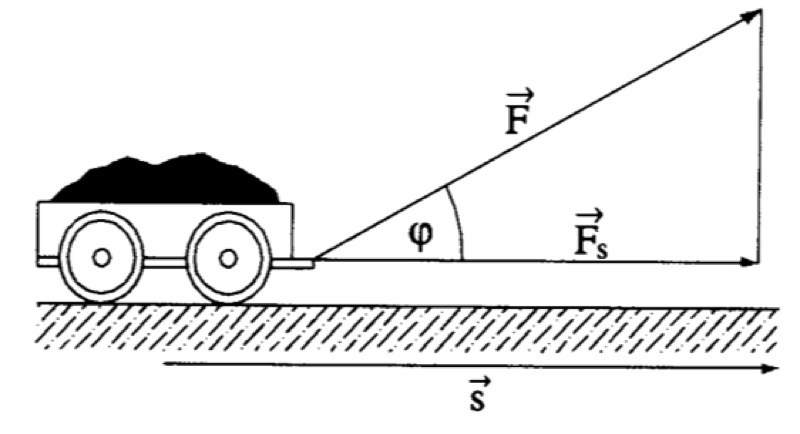
\includegraphics[width=0.49\textwidth]{pictures/arbeit}
\end{center}
\caption{Arbeit ist \glqq Kraft mal Weg\grqq}
\end{figure}

Benutzt man $F_s = F\cdot\cos\varphi$, so erhält man für die Arbeit
$$W = \V{F_s}\cdot\V{s} = F\cdot s \cdot \cos \varphi$$
Merkwürdig ist, dass die Verknüpfung zweier vektorieller Grässen (Kraft, Weg) eine skalare Grösse (Arbeit) ergibt. Ferner bemerken wir, dass die Länge von $\V{F_s}$ vom Winkel $\varphi$ abhängt.

\section{Zerlegung eines Vektors}
Die Zerlegung eines beliebigen Ortsvektors nach den Basisvektoren $\ex$ und $\ey$ im rechtwinkligen Koordinatensystem ist ein Spezialfall eines allgemeineren Sachverhalts. Insbesondere bei physikalischen Problemen muss man oft eine Kraft in zwei Teilkräfte, deren Richtungen vorgegeben sind, zerlegen.

\begin{bsps}
\ \\[-4ex]
\begin{itemize}
\item Die Lampe einer Strassenbeleuchtung hängt an zwei Spannseilen. Die Gewichtskraft der Lampe wird in zwei Teilkräfte mit vorgeschriebenen Richtungen zerlegt.
\item Eine Kugel mit der Gewichtskraft $\V{F_G}$ bindet sich auf einer schiefen Ebene mit Neigungswinkel $\ga$. $\V{F_G}$ lässt sich in die beiden Teilkräfte Hangabtriebskraft $\V{F_H}$ und Normalkraft $\V{F_N}$ zerlegen.
\end{itemize}
\end{bsps}

\begin{ueb}[Keil erforderlich?]
Eine $\unit[120]{m}$ lange Strasse steigt um $\unit[18]{m}$ an; auf ihr steht ein $\unit[42]{kN}$ schwerer Lastzug. Welche Kraft ist erforderlich, um ein Abwärtsrollen zu verhindern?
\end{ueb}
\section{Realistische Darstellungen mit dem Computer}
Wer kennt sie nicht, die Computergraphiken und -animationen in den Videoclips, in der Werbung, in kommerziellen und wissenschaftlichen Filmen, \dots?

\begin{itemize}
\item In einem Werbespot der Firma General Motors wird ein Sportwagen vom Typ Pontiac Fiero Bauteil für Bauteil über den Wolken montiert.
\item Für das Weltraum-Epos \glqq The Last Starfighter\grqq\ wurden im Computer --- ohne Modelle oder Zeichentrick-Vorlagen --- 27 Minuten Schlachtgetümmel und Sternreisen komponiert.
\item Die Digital Effects Studios in New York bauten im Computer einen Strassenzug Manhattans der 30er Jahre nach, in dem der Betrachter mit naturgetreu wechselnden Perspektiven zwischen Wolkenkratzern wandeln kann.
\item Am MIT wurde ein Computer-Trickfilm entwickelt, in dem ein nahezu lichtschnelles Raumschiff den Studenten die Tücken relativistischer Raumfahrt demonstriert.
\end{itemize}

Um wirklichkeitsgetreue Abbildungen zu erhalten, muss man die verschiedensten Dinge beachten wie zum Beispiel die Richtung des einfallenden Lichts, die Ober\-flä\-chen\-be\-schaf\-fen\-heit der darzustellenden Körper, deren Licht\-durch\-läs\-sig\-keit etc. In Wirklichkeit sind sehr wenige Flächen einfarbig. Oft beeinflussen Schattierungen, Spiegelbilder und durchscheinende Bilder das Ergebnis. Mit einfachen und komplizierten Algorithmen kann man heute schon sehr realistische Bilder erstellen. Im folgenden Abschnitt wird gezeigt, wie eine Tiefenwirkung durch die verschiedenen Be\-gren\-zungs\-flächen eines Körpers mit einer einfachen Idee erzeugt werden kann.

\begin{figure}
\begin{center}
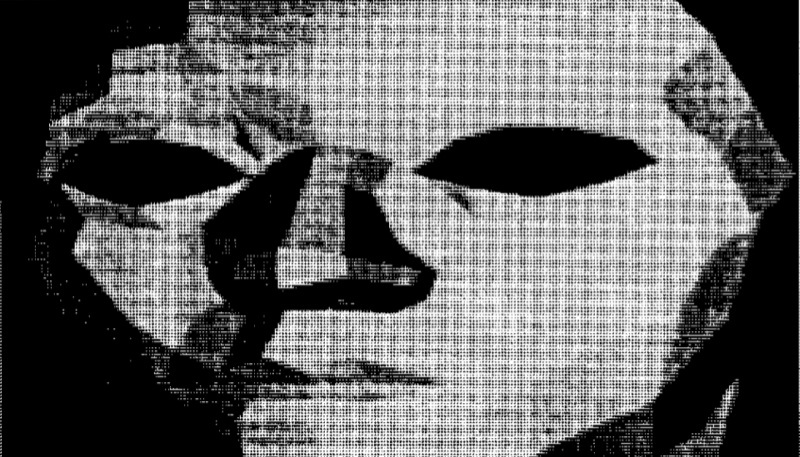
\includegraphics[width=0.7\textwidth]{pictures/pcgrafik}
\end{center}
\caption{Polygonmodell eines Kopfs}
\end{figure}

Wir gehen davon aus, dass der darzustellende Körper von einer Lichtquelle, die sich der Einfachheit halber im Unendlichen befindet, beleuchtet wird. Die Lichtstrahlen treffen auf die verschiedenen Begrenzungsflächen des Körpers auf und werden nach dem Reflexionsgesetz (Einfallswinkel=Ausfallswinkel) reflektiert.

\begin{figure}
\begin{center}
\definecolor{qqwuqq}{rgb}{0,0.39,0}
\definecolor{zzttqq}{rgb}{0.6,0.2,0}
\scalebox{0.8}{
\begin{tikzpicture}[line cap=round,line join=round,>=triangle 45,x=0.8cm,y=1.0cm]
\clip(-4.3,-0.72) rectangle (4.28,6.3);
\fill[color=zzttqq,fill=zzttqq,fill opacity=0.1] (-3.96,4.32) -- (-3,5) -- (0.72,-0.02) -- (-0.68,0) -- cycle;
\draw [shift={(-1.28,2.68)},color=qqwuqq,fill=qqwuqq,fill opacity=0.05] (0,0) -- (35.2:2) arc (35.2:51.25:2) -- cycle;
\draw [shift={(-1.28,2.68)},color=qqwuqq,fill=qqwuqq,fill opacity=0.05] (0,0) -- (20.87:2) arc (20.87:35.2:2) -- cycle;
\draw [color=zzttqq] (-3.96,4.32)-- (-3,5);
\draw [color=zzttqq] (-3,5)-- (0.72,-0.02);
\draw [color=zzttqq] (0.72,-0.02)-- (-0.68,0);
\draw (-1.28,2.68)-- (2.86,5.6);
\draw (-1.28,2.68)-- (1.4,6.02);
\draw (-1.28,2.68)-- (3.18,4.38);
\draw [->] (1.4,6.02) -- (0.02,4.3);
\draw [->] (-1.28,2.68) -- (0.8,3.47);
\draw[color=qqwuqq] (0,3.8) node {$\varphi$};
\draw[color=qqwuqq] (0.3,3.5) node {$\varphi$};
\end{tikzpicture}
}
\end{center}
\caption{Lichtreflexion an glatter Oberfläche}
\end{figure}

Man nimmt nun an, dass die Helligkeit einer Fläche nur durch den Einfallswinkel $\varphi$ bestimmt wird. In der Informatik benutzt man die \emph{Lambert'sche Regel}, die besagt, dass der Anteil des jeweils reflektierten Lichts gleich dem Cosinus des Einfallswinkels $\varphi$ ist.
Wenn $L$ die Intensität der Lichtquelle ist, so berechnet sich die Helligkeit $H$ der darzustellenden Fläche durch
$$H(\varphi)=k\cdot L\cdot\cos(\varphi)$$
wobei $k$ eine Materialkonstante ist. $k$ nimmt Werte zwischen $0$ und $1$ an und gibt den Prozentsatz des reflektierten Lichts an.

Mit Hilfe dieser einfachen Methode kann man mit verhältnismässig wenig Rechenaufwand schon erstaunlich gute Bilder erstellen.

\begin{ueb}[Lambert]
Der abgebildete Würfel wird aus der Richtung
$$\vec{v}=\pV{-3}{-2}{-1}$$
bestrahlt. Berechne für $k=0.5$ und $L=1$ die Helligkeiten, mit der die drei beleuchteten Würfelflächen eingefärbt werden sollen. Färbe die drei Flächen mit drei verschiedenen Grautönen ein.
\begin{center}
\scalebox{0.8}{
\begin{tikzpicture}[line cap=round,line join=round,>=triangle 45,x=0.8cm,y=0.8cm]
\clip(-4.3,-0.76) rectangle (6.12,6.3);
\draw [->,dash pattern=on 2pt off 2pt] (-3,1) -- (4.5,1);
\draw [->,dash pattern=on 2pt off 2pt] (-1,0) -- (-1,6);
\draw [->,dash pattern=on 2pt off 2pt] (0.3,1.66) -- (-4.06,-0.54);
\draw (-3,0)-- (1,0);
\draw (1,0)-- (3,1);
\draw (-3,0)-- (-3,4);
\draw (1,0)-- (1,4);
\draw (3,1)-- (3,5);
\draw (-3,4)-- (-1,5);
\draw (-3,4)-- (1,4);
\draw (1,4)-- (3,5);
\draw (-1,5)-- (3,5);
\draw (-3,0)-- (-1,1);
\draw (-1,1)-- (-1,5);
\draw (-1,1)-- (3,1);
\draw (-3.7,0.5) node[anchor=north west] {1};
\draw (3.2,1.6) node[anchor=north west] {1};
\draw (-1.5,5.7) node[anchor=north west] {1};
\end{tikzpicture}
}
\end{center}
\end{ueb}

\begin{figure}[ht]
\begin{center}
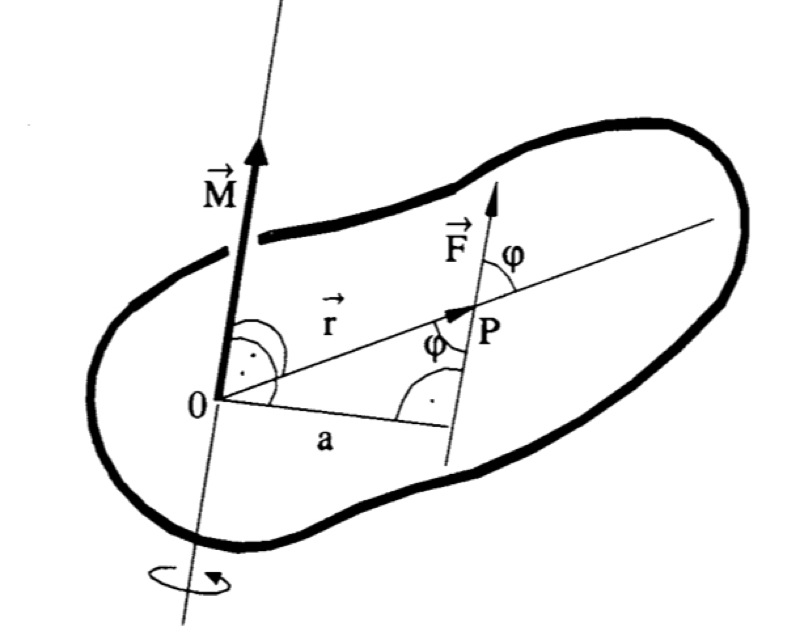
\includegraphics[width=5cm]{pictures/vprodukt}
\end{center}
\caption{Drehmoment $\V{M}$}\label{abb:vektorprod}
\end{figure}

Auf den Körper wirke im Punkt $P$ eine Kraft $\V{F}$ wie in Abbildung \ref{abb:vektorprod} auf Seite \pageref{abb:vektorprod} skizziert. Für die Berechnung des Drehmoments $M$ benötigt man nicht die Entfernung $r =\overline{OP}$, sondern den Abstand $a =r\cdot\sin\varphi$ der Wirkungslinie der Kraft vom Drehpunkt $O$:
$$M =a\cdot F =r\cdot F\cdot \sin\varphi$$

Physikalische Experimente zeigen:
\begin{itemize}
\item die Drehachse steht senkrecht zur Ebene, die durch
$\V{r}$ und $\V{F}$ aufgespannt wird,
\item die Drehrichtung wird durch $\V{r}$ und $\V{F}$ so bestimmt,
dass ein rechtshändiges System vorliegt ($\V{r}$: Daumen,
$\V{F}$: Zeigefinger, Drehrichtung: Mittelfinger der rechten Hand).
\end{itemize}
Man schreibt dafür:
$$\V{M}=\V{r}\times\V{F}$$
(lies: \glqq $r$ Kreuz $F$\grqq)

\begin{bsp}
Eine nützliche Anwendung zeigt sich in der Elektrotechnik zur Bestimmung der Richtung der Lorentzkraft. Es gilt nämlich
$$\vec{F}=Q\cdot(\vec{v}\times\vec{B}),$$
wobei $Q$ für die Ladung, $\vec{v}$ für die Geschwindigkeit der Ladung und $\vec{B}$ für das Magnetfeld steht.
\begin{figure}
\begin{center}
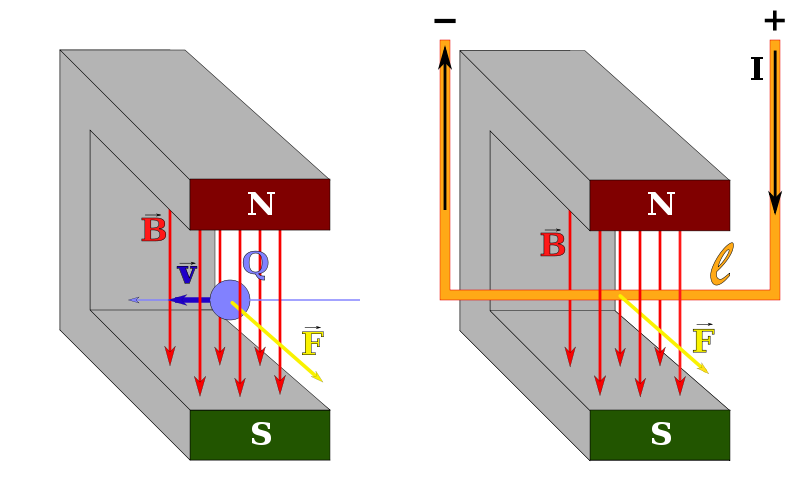
\includegraphics[width=0.4\textwidth]{pictures/lorentz.png}
\caption{Lorentzkraft $\vec{F}$}
\end{center}
\end{figure}
Der ausgestreckte rechte Zeigefinger folgt der technischen Stromrichtung, also der Bewegungsrichtung von positiv geladenen Ladungsträgern bzw. der entgegengesetzten Bewegungsrichtung negativer Ladungsträger.
Der ausgestreckte rechte Mittelfinger folgt der Richtung der Magnetfeldlinien, also der Richtung, in die sich der Nordpol eines Probemagneten ausrichtet.
Der rechte Daumen zeigt nun in die Wirkungsrichtung der Lorentzkraft.
\end{bsp}

\cleardoublepage

\listoffigures

\end{document}
